\newpage
\chapter{Background Theory and Method}
% \addcontentsline{toc}{chapter}{Background Theory and Method} 

Small introtext to motivate this chapter. What am I going to go over here.


\section{Tribology - friction}

% (from wikipedia so far: https://en.wikipedia.org/wiki/Friction)

% the elementary processes of dry, wearless surface sliding 

% Terms: mesoscale: Of medium size or extent; between microscale and macroscale

% Quotes: Sliding friction that takes place between two surfaces in the absence of lubricant is termed "dry" friction even if the process
% occurs in an ambient environment. (Nanotribology and Nanomechanics, p. 329)


% For monolayers sliding along atomically uniform substrates, however, there is essentially no static friction. Indeed, the friction in
% these systems can be up to 105 times less than that for macroscopic lubricants such as graphite. This raises questions about the
% fundamental dissipation mechanisms that are at work in systems at different scales.
% (\url{https://physicsworld.com/a/friction-at-the-nano-scale/})

% The trouble is that the coefficients of friction measured in nanotribological experiments and in macroscopic “tribotests” routinely differ
% by orders of magnitude. (\url{https://physicsworld.com/a/friction-at-the-nano-scale/})

% We were astonished to discover that molecules that could flex or slide even just a little in response to the oscillatory motion of the
% microbalance were linked to low friction levels at the macro-scale. Put another way, exceptionally low friction at the atomic scale was
% not a prerequisite for the substantial reduction in macroscopic friction. (\url{https://physicsworld.com/a/friction-at-the-nano-scale/})


% At face value, the transition from a static strained configuration to full sliding is conceptually as simple as overcoming an energy
% barrier. However, practical single- and multiple- contact conditions are characterized by complex interaction profiles plus nontrivial
% internal dynamics. As a result, the interplay of thermal drifts, contact ageing, contact-contact in- teractions, and macroscopic elastic
% deformations introduce significant complications, and make the depinning transition from static to kinetic friction an active field of
% research. The depinning dynamics affects in particular the transition between stick-slip and smooth slid- ing for sliding friction.
% (Current trends in the physics of nanoscale friction)

% In Atomic Force Microscopy (AFM) experiments, when the tip scans over the monolayers at low speeds, friction force is reported to increase
% with the logarithm of the velocity, similar to that observed when the tip scans across crystalline surfaces. This velocity dependence is
% interpreted in terms of thermally activated depinning of interlocking barriers involving interfacial atoms. (Current trends in the physics
% of nanoscale friction)

% Da Vinci-Amontons law – friction independent of area – is not confirmed at the microscopic scale. In most nanoscale investigations the
% friction of a single con- tact is found to increase linearly with the contact area [27–29]. In contrast, structurally mismatched
% atomically flat and hard crystalline or amorphous surfaces are expected to produce a sublinear increase of friction with contact area. The
% frequent finding of friction proportional to area even in some of these cases can be understood as a consequence of softness, either if
% the interface, or of surface contaminants leading to effectively pseudo- commensurate interfaces [30, 31] (Current trends in the physics
% of nanoscale friction)


% \begin{itemize} \item Amontons' First Law: The force of friction is directly proportional to the applied load. \item Amontons' Second Law:
%     The force of friction is independent of the apparent area of contact. \item Coulomb's Law of Friction: Kinetic friction is independent
%     of the sliding velocity. \end{itemize} Columbd friction \begin{align*} F_f \le \mu F_n \end{align*}


% The study of friction, wear and lubrication between two surfaces in relative motion is called tribology. \cite{gnecco_meyer_2015}.

% We will limit ourself to the elementary processes of dry, wearless surface sliding. In general we can divide friction in to two scales:
% Macroscopic and microscopic, for which the properties turns out to differ quite substantially.  

% Make an explicit distinction between macroscale and microscale. Get some numbers on it!

% Sliding friction that takes place between two surfaces in the absence of lubricant is termed ``dry''  friction even if the process occurs
% in an ambient environment. (Nanotriology and Nanomechanics, p. 329)



% The differences between the conventional or macrotribology and micro/nanotribology are contrasted in Figure 1.3.1. In macrotribology,
% tests are conducted on components with relatively large mass under heavily loaded conditions. In these tests, wear is inevitable and the
% bulk prop- erties of mating components dominate the tribological performance. In micro/nanotribology, measurements are made on components,
% at least one of the mating components, with relatively small mass under lightly loaded conditions. In this situation, negligible wear
% occurs and the surface properties dominate the tribological performance. \cite{bhushan_2013}[p. 5]


% It is generally accepted that friction is caused by more than one mechanism in a given sliding system. Generally, frictional force arises
% due to two fundamentally different causes, namely one that is mechanical in nature and the other being chemical in its origin. In the case
% of mechanical cause of friction, plowing of the surface by hard particles or asperities is mainly responsible for generating the
% frictional force.2,4,5-7 As for the chemical mechanism of friction, adhesion between surfaces of the two solids in contact is the cause of
% friction.2,4,5,8 Another point to note is that tribological phenomena are heavily dependent on system parameters of the operating machine
% such as speed, temperature, load, and environment. As such, the dominating. \cite{kim_nano-scale_2009}.


% Tribological systems pose a wide range of dimensional scale. At the largest scale, geological stratum layers that are involved in
% earthquakes may be considered as a tribological system. The movement of the stratum occurs when the frictional forces between the layers
% are overcome by internal pressure inside the earth. At the smallest scale, relative motion of atoms at the interface of two materials
% would be a good example that involves frictional interaction. Owing to the vast difference in scale, the dominant mechanisms of friction
% and wear in macro-scale systems may be different from those of micro/nano-scale systems. In macro-scale, the tribological systems
% experience relatively large contact stresses and speeds. On the other hand, micro/nano-scale systems operate under relatively low loads
% and speeds. Particularly, the inertial effects that are prominent in macro-scale may be insignificant at the micro/nano-scale. Rather,
% surface forces often dictate the tribological interactions at small scales. \cite{kim_nano-scale_2009}.


% Experimental research to examine the frictional characteristics at the atomic-scale has been conducted for the past two decades. It is
% well known that frictional behavior cannot be generalized by a few factors such as normal load, surface roughness, speed, and material
% type of the tribological system. Other conditions such as temperature, humidity, and even sliding history can affect the tribological
% phenomena significantly. Particularly at nano-scale, the tribological behavior tends to be more sensitive to the state of outermost layer
% of the surface region. Thus, contamination layer, adsorbed gas, capillary junctions, and oxide layer become more important at small
% scales. This is because at nano-scale the contact forces are often too low for the asperities to penetrate the surface layers and the
% magnitude of the surface force may be comparable to the frictional force. {kim_nano-scale_2009}.

% The first well known studies of friction concerns itself is based on a macroscopic level. That is, the scale of visible everyday objects.
\subsection{Friction on a macroscopic scale - macroscale theories}
\subsubsection {Amontons’ law. }
 The work of Leonardo da Vinci (1452–1519), Guillaume Amontons (1663-705) and Charles de Coulomb (1736-1806) all contributed to what is
 commonly known as Amontons’ law describing the frictional force accuring when starting and keeping a solid block sliding against a solid
 surface. This emperical law states that the frictional force tangential to the sliding direction is entirely independent of contact area
 and sliding velocity (at ordinary sliding velocities). Instead it relies only on the normal force $F_N$ acting from the surface on the
 block and the material specific friction coefficient $\mu$ as
\begin{align*}
  F_f = \mu F_N.
\end{align*}

Further it distinguish between \textit{static} and \textit{kinetic} friction as the cases of stationary and sliding contact resepectively.
Each type of friction comes with its own friction coefficient, $\mu_s$ for static and $\mu_k$ for kinetic friction, usually with values
lower than one and $\mu_s \ge \mu_k$ in all cases. \cite{gnecco_meyer_2015}[p. 6]. \\

This simple law is a natural starting point for the

Allthough this model is a common base for understanding friction on a macroscopic level is has its limitations. It turns out that static
friction is not constant, but depends on the so-called contact history with increasing friction as the logarithm of time of stationary
contact \cite{dieterich_1972}. For the kinetic friction the independency of sliding velocity dissapears at low velocities as thermal effects
becomes important and for high velocities due to intertial effetcs. \cite{gnecco_meyer_2015}[pp. 5-6]. \\

It fails to explain the mechanisms behind fritction.
 

In order to understand what is causing friction between moving objects and how this might result in a linear relationship between friction
and normal force we must take the study to a smaller scale... Having an emperical law that seems to predict the friction in many cases leads
to the next natural desire for deriving these from fundamental atomic or molecular principles.

\subsection{Friction on a microscopic scale - Nanotribology}
It is generally accepted that friction is caused by two mechanism: mechanical friction and chemical friction. The mechanical friction is the
plowing of the surface by hard particles or asperities. The chemical mechanism is adhesion between contacting surfaces.
\cite{kim_nano-scale_2009}.


Sources in general: \cite{mo_friction_2009}, \cite{kim_nano-scale_2009} \\

\subsubsection{Surface roughness - Asperity theories}

Going beyond a macroscopic perspective we realise that most surfaces is in fact rough. The contact between two surfaces consist of numerous
smaller contact point, so-called asperities, each with a contact area of $A_{\text{asp}}$. The true contact area $\sum A_{\text{asp}}$ is
found to be much smaller than the apperent macroscopic area $A_{\text{macro}}$. The friction force is shown to be proportional (extra source
on this) to this true contact area as 

\begin{align*}
  F_f = \vec{\tau} \sum A_{\text{asp}},
\end{align*}

where $\vec{\tau}$ is an effective shear strength of the contacting bodies. This is still compatible with Amontons’ law as long as we
differenciate between the macroscopic macroscopic and true area and by having the true contact area dependt linearly on applied normal
force. \\

Thus many studies have focused individual asperities to reveal the relationship between the contact area and normal force  (13-15 from
\cite{mo_friction_2009}). By assuming perfectly smooth asperities with radii of curvature from nanometers to micrometres in size continuum
mechanics can be used to predict the deformation of asperities as normal force is applied. A model for non-adhesive contact between
homogenous, isotropic, linear elastic spheres was first developed by Hertz (17 \cite{mo_friction_2009}), which predicted $A_{\text{asp}}
\propto F_N^{2/3}$. Later adhesion effects were included in a number of subsequent models, including Maugis-Dugdale theory (18 from
\cite{mo_friction_2009}), which also predicts a sublinear relatinship between $A_{\text{asp}}$ and $f_N$ leading to a similar sublinear
relationship for $F_f$ and $F_N$.

% Picture of asperities from wiki: https://en.wikipedia.org/wiki/Asperity_%28materials_science%29#/media/File:Asperities.svg
\cite{mo_friction_2009}.

% However, practical single- and multiplecontact conditions are characterized by complex interaction profiles plus nontrivial internal
% dynamics. As a result, the interplay of thermal drifts, contact ageing, contact-contact interactions, and macroscopic elastic deformations
% introduce significant complications, and make the depinning transition from static to kinetic friction an active field of research.
% \cite{Manini_2017}[p. 2]. 



\subsubsection{Atomic level friction }
On the smallest possible scale, atomic scale, the surfaces does not have structural asperities. Instead atomic level friction is being model
as a consequencse of the rough potential of the atomic landscape. 

\subsubsection{Frenkel-Kontorova-Tomlinson (FKT)}
Describes atomic scale friction (not fully accurately though) and gives insight in stick slip motion. 



\subsubsection{Commensurate and incommensurate}
\subsubsection{Stick slip}



At nanoscales things get a bit more unclear. SFM (explain) experiments have reported (copy sources 5, 6, 21 from \cite{mo_friction_2009})
where $F_f \propto F_N$ or even with these quantities being nearly independent of each other.



% \cite{physicsworld_2005}





In several works by J. Fineberg’s group [2–4] the transition from sticking to sliding is characterized by slip fronts propagating along the
interface. \cite{Manini_2017}[p. 2]. 

\subsubsection{Commensurate and incommensurate}
As expected, high levels of friction were present in the commensurate positions and extremely low friction was found when the surfaces were
incommensurate. (\url{https://physicsworld.com/a/friction-at-the-nano-scale/})


\subsubsection{Superlubricity?}
Superlubricity, now a pervasive concept of modern tribology, dates back to the math- ematical framework of the Frenkel Kontorova model for
incommensurate interfaces [40]. When two contacting crystalline workpieces are out of registry, by lattice mismatch or angular misalignment,
the minimal force required to achieve sliding, i.e. the static friction, tends to zero in the thermodynamic limit – that is, it can at most
grow as a power less than one of the area – provided the two substrates are stiff enough. (Current trends in the physics of nanoscale
friction)


Superlubricity is experimentally rare. Until recently, it has been demonstrated or im- plied in a relatively small number of cases [29,
42–46]. There are now more evidences of superlubric behavior in cluster nanomanipulation [32, 33, 47], sliding colloidal layers [48–50], and
inertially driven rare-gas adsorbates [51, 52]. (Current trends in the physics of nanoscale friction)


A breakdown of structural lubricity may occur at the heterogeneous interface of graphene and h-BN. Because of lattice mismatch (1.8\%), this
interface is intrinsically incommen- surate, and superlubricity should persist regardless of the flake-substrate orientation, and become
more and more evident as the flake size increases [57]. However, vertical cor- rugations and planar strains may occur at the interface even
in the presence of weak van der Waals interactions and, since the lattice mismatch is small, the system can de- velop locally commensurate
and incommensurate domains as a function of the misfit angle [58, 59]. Nonetheless, spontaneous rotation of large graphene flakes on h-BN is
observed after thermal annealing at elevated temperatures, indicative of very low friction due to incommensurate sliding [60, 61]. (Current
trends in the physics of nanoscale friction)

Indeed, we know from theory and simulation [74–76] that even in clean wearless friction experiments with perfect atomic structures,
superlubricity at large scales may, for example, surrender due to the soft elastic strain deformations of contacting systems. (Current
trends in the physics of nanoscale friction)




\subsection{Temperature dependence}
Thus, it is commonly expected that the friction of a dry nanocontact should classically decrease with increasing temperature provided no
other surface or material parameters are altered by the temperature changes [77, 80–83]. (Current trends in the physics of nanoscale
friction)


\subsection{Summary of expected frictional properties}
\begin{enumerate}
  \item Friction should decrease by increasing temperature.
  \item We expect stick slip motion
  \item What about dependence on normal force?
  \item Dependence on contact area?
  \item Dependense on speed? 
\end{enumerate}

\begin{itemize}
  \item Different friction models on macro-and microscopic scale
\end{itemize}
\subsection{Graphene}
Because of this frictional reduction, many studies indicate graphene as the thinnest solid-state lubricant and anti-wear coating [104–106].
(Current trends in the physics of nanoscale friction)


Accurate FFM measurements on few-layer graphene systems show that friction decreases by increasing graphene thickness from a single layer up
to 4-5 layers, and then it approaches graphite values [97, 99, 101, 107, 108]. (Current trends in the physics of nanoscale friction)



\begin{itemize}
  \item General properties and crystal structure
\end{itemize}
\subsection{Molecular Dynamics}



\subsubsection{Potentials}
% \cite{PhysRevB.37.6991}
The choices of potentials is mainly based on the on \cite{li_evolving_2016}. The covalent bonds of C-C in graphene and Si-Si in the substrate is described by the Tersoff and Stillinger–Weber potentials, respectively. A typical 6–12 Lennard–Jones potential is used to describe the van der Waals adhesive interaction between graphene and the substrate. 


Quantum-mechanical calculations is more accurate but to numerical intensive.


Despite recent progress in this respect, it is clear that there will always be interesting problems beyond the reach of ab initio approaches \cite{PhysRevB.37.6991}.

In particular, pair potentials are completely inapplicable to strongly co- valent systems such as semiconductors \cite{PhysRevB.37.6991}.

Pair potentials comes from the following expansion. The energy of $N$ interacting particles may be written 
\begin{align*}
  E = \sum_i V_1(\vec{r}_i) + 
      \sum_{\substack{i, j \\ i < j}} V_2(\vec{r}_i, \vec{r}_j) +  
      \sum_{\substack{i,j,k \\ i < j < k}} V_3(\vec{r}_i, \vec{r}_j, \vec{r}_i) + \cdots,
\end{align*}
% \sum_{\substack{i=0 \\ i\neq 4}}^n i
% \begin{align*}
%   E = \sum_i V_i(\vec{r}_i) + \sum_i\sum_{j>i} V_2(\vec{r}_i, \vec{r}_j) +  \sum_i\sum_{j>i}\sum_{k>j} V_3(\vec{r}_i, \vec{r}_j, \vec{r}_i) + \cdots,
% \end{align*}
where $\vec{r}_n$ is the position of the $n$th particle and $V_m$ is called an $m$-body potential.
The first one-body term corresponds to an external potential, followed by the two-body term, three-body term an so on. The simplest model that includes parrticle interaction is the pair potential truncating the expansion after the two-body term. A general feature of the pair potentials is that they favor close-packed structures which is unsuited to describe covalent bonds that take more open structures. In order to accomodate the description of covalent bonds the natural step is to include the next step of the expansion, the three-body terms. 

\subsubsection{Leonard Jones}



\subsubsection{Stillinger weber}
% https://docs.lammps.org/pair_sw.html
% \cite{PhysRevB.31.5262}

The stillinger weber potential takes the form of a three body potential
\begin{align*}
  E &=\sum_i \sum_{j>i} \phi_2(r_{i j})+\sum_i \sum_{j \neq i} \sum_{k>j} \phi_3(r_{ij}, r_{ik}, \theta_{ijk}).
\end{align*}
The two-body term $\phi_2$ builds from the Lennard-Jones (LJ) model with the addition of an exponetial term
\begin{align*}
  \phi_2(r_{i j}) & =A \epsilon_{ij}\left[B\left(\frac{\sigma}{r_{ij}}\right)^{p_{ij}} - \left(\frac{\sigma}{r_{ij}}\right)^{q}\right] \exp (\frac{\sigma}{r_{ij}-a \sigma}).
\end{align*}

The model parameters $A$, $\epsilon$, $B$, $\sigma$, $p$, $q$ and $a$ should be specified for each unique atom type pair, but since we are only dealing with Si-Si bonds we can exclude the $i,j$ indices on thoose. We see that the first term is reminiscent of the Lennard-Jones potential while the last term forces the potential to zero at $r=a\sigma$.

\begin{align*}
  \phi_3(r_{ij}, r_{ik}, \theta_{ijk}) &= \lambda \ \epsilon \Big[\cos \theta_{ijk}-\cos \theta_{0,ijk}\Big]^2 \exp (\frac{\gamma \sigma}{r_{ij} - a \sigma}) \exp (\frac{\gamma \sigma}{r_{ik} - a \sigma}).
\end{align*}
Similar here the added model parameters should be defined for all unique triplets of atom types. 

%%%%%%%%%%%%%%%%
%%%%%%%%%%%%%%%%
%%%%%%%%%%%%%%%%
% WORKING HERE
%%%%%%%%%%%%%%%%
%%%%%%%%%%%%%%%%
%%%%%%%%%%%%%%%%

% and three-body term $\phi_3$ takes respectively take the form
% \begin{align*}
%   \phi_2(r_{i j}) & =A_{ij} \epsilon_{ij}\left[B_{ij}\left(\frac{\sigma_{ij}}{r_{ij}}\right)^{p_{ij}} - \left(\frac{\sigma_{ij}}{r_{ij}}\right)^{q_{ij}}\right] \exp (\frac{\sigma_{ij}}{r_{ij}-a_{ij} \sigma_{ij}}), \\
%   \phi_3(r_{ij}, r_{ik}, \theta_{ijk}) &= \lambda_{ijk} \ \epsilon_{ijk}\Big[\cos \theta_{ijk}-\cos \theta_{0,ijk}\Big]^2 \exp (\frac{\gamma_{ij} \sigma_{ij}}{r_{ij}-a_{ij} \sigma_{ij}}) \exp (\frac{\gamma_{ik} \sigma_{ik}}{r_{ik}-a_{ik} \sigma_{ik}}).
% \end{align*}
$r_{ij}$ denotes the distance between atom $i$ and $j$ and $\theta_{ijk}$ the angle between bond $ij$ and $jk$. The summations is over all neighbours $j$ and $k$ of atom $i$ within a cutoff (decide about ``-'' or not) distance  $a/\sigma$? (cutoff: r = a)? The indices for $\sigma, p, q, a, \lambda$ denotes the oppoertunity to specify different parameters for different atom types. In our case this is not used as this will only model Si-Si interactions. 




$\epsilon$ is the depth of the potential well (LJ). $\sigma$ is the distance at which the potential is zero


\begin{table}[H]
  \begin{center}
  \caption{Parameters for the stilliner weber potential used for intermolecular interactions in the silicon substrate}
  \label{tab:param}
  \begin{tabular}{ | c | c | c|} \hline
    Parameter & Value & Description \\ \hline 
    $\epsilon$ & 2.1683  & ... \\ \hline
    $\sigma$ & 2.0951 & ... \\ \hline
    $a$ & 1.80 & ... \\ \hline
    $\lambda$ & 21.0 & ... \\ \hline
    $\gamma$ & 1.20 & ... \\ \hline
    $\cos{(\theta_0)}$ & -1/3 & Equilibrium angle \\ \hline
    $A$ &  7.049556277 & \\ \hline
    $B$ &  0.6022245584 &  \\ \hline
    $p$  & 4.0 & \\ \hline
    $q$  & 0.0 & \\ \hline
    $tol$  & 0.0 & \\ \hline
  \end{tabular}
  \end{center}
\end{table}


% #   element 1, element 2, element 3,
% #   epsilon, sigma, a, lambda, gamma, costheta0, A, B, p, q, tol

% Si Si Si 
% eps2.1683  sigma2.0951  a1.80  lambda21.0  gamma1.20  -0.333333333333 A7.049556277  0.6022245584  4.0  0.0 0.0

\subsubsection{Tersoff}
% https://docs.lammps.org/pair_tersoff.html
% https://chem.libretexts.org/Bookshelves/Physical_and_Theoretical_Chemistry_Textbook_Maps/Supplemental_Modules_(Physical_and_Theoretical_Chemistry)/Chemical_Bonding/Fundamentals_of_Chemical_Bonding/Bond_Order_and_Lengths
% https://en.wikipedia.org/wiki/Bond_order_potential


% https://interatomic-potentials.readthedocs.io/en/latest/doc/tersoff.html
% \cite{PhysRevB.37.6991}

The tersoff potential abandon the idea of a general $N$-body form and attempts instead to build the model on a more physics informed approach. The more neighbours an atom has the weaker the bonds will be. Thus it introduces the bond order (bond strentgh), that is environment specific and increase with bond coordination (number of neighbours for a given atom). The potential energy is taken to have the form

\begin{align*}
  E &= \sum_i E_i = \frac{1}{2}\sum_{i \ne j} V_{ij}, \\
  V_{ij} &= f_C(r_{ij}) \big[f_R(r_{ij}) + b_{ij}f_A(r_{ij})  \big],
\end{align*}

% where the total potential energy is decomposed into an atom site energy $E_i$ and a bond energy $v_{ij}$. 
where the total potential energy is decomposed into a bond energy $V_{ij}$. The indices $i$ and $j$ run over the atoms of the system with $r_{ij}$ denoting the distance between atom $i$ and $j$. The bond energy is composed of a repulsive term $f_R$, arising from overlapping wave functions, and a attractive term $f_A$ associated with bonding. $f_c$ is simple a smooth cut-off function to increase computational efficiency. $b_{ij}$ represent the bond order, i.e. the strength of the bonds, which depends inversely on the number of bonds, the bond angles ($\theta_{ijk}$) and optionally the relative bonds lengths ($r_{ij}$, $r{jk}$). Notice that an additional cut-off term $a_{ij}$ was orginally multiplied to $f_R$ as a way of including terms that limit the range of the interactions to the first neighbour shell. These kind of limitations is already included in $b_{ij}$ for the attractive term $f_A$ but is often omitted for the repulsive term $f_R$ and we do so by setting $a_{ij} = 1$. \\
The cut-off function goes from 1 to 0 over a small interval range $R \pm D$ as
\begin{align*}
  f_C(r) =
  \begin{cases}
    1 & r < R - D \\
    \frac{1}{2} - \frac{1}{2} \sin{(\frac{\pi}{2} \frac{r - R}{D})} & R - D < r < R + D\\
    0 & r > R + D
  \end{cases},
\end{align*}
which is continuous and differentiable for all $r$. $R$ is usually chosen to include only the first neighbour shell. \\
The repulsive and attractive terms $f_R$ and $f_A$ is modelled as an exponetial function, just as in a morse potential, 
\begin{align*}
 f_R(r) &= A \exp(-\lambda_1 r), \\
 f_A(r) &= -B \exp \big(-\lambda_2 r\big),
\end{align*}


The novel feature of the model lies in modeling of the bond order $b_{ij}f_A$ which includes a three-body interactions by summing over a third atom $k \ne i,j$ within the cut-off $r_{ik} < R + D$.

\begin{align*}
  b_{i j} & =\big(1+\beta^n \zeta_{i j}^n\big)^{-\frac{1}{2 n}} \\
  \zeta_{i j} & =\sum_{k \ne i,j} f_C(r_{i k}) g\Big(\theta_{i j k}\left(r_{i j}, r_{i k}\right)\Big) \exp \left(\lambda_3{ }^m\big(r_{i j}-r_{i k}\right)^m\big) \\
  g(\theta) & =\gamma_{i j k}\left(1+\frac{c^2}{d^2}-\frac{c^2}{\left[d^2+\left(\cos \theta-\cos \theta_0\right)^2\right]}\right)
\end{align*}

$\zeta_{i,j}$ is effective coordination and $g(\theta)$ is minimized at the equilibrium angle $\theta = \theta_0$.
% and considering the angle $\theta_{ijk}$, that is the angle between bonds $r_{ij}$ and $r_{jk}$.




\begin{table}[H]
  \begin{center}
  \caption{Parameters for the tersoff potential used for intermolecular interations in the graphene sheet}
  \label{tab:param}
  \begin{tabular}{ | c | c | c|} \hline
    Parameter & Value & Description \\ \hline 
    $m$ & 3.0 & Default (not used since $\lambda_3 = 0$ ) \\ \hline
    $\gamma$ & 1.0 & \\ \hline
    $\lambda_3$ & 0.0 Å$^{-1}$ & \\ \hline
    $c$ & \num{3.8049e4} & Strength of the angular effect \\ \hline
    $d$ & 4.3484 & Determines the ``sharpness'' of the angular dependency \\ \hline
    $\cos{(\theta_0)}$ & -0.57058  & \\ \hline
    $n$ & 0.72751 & \\ \hline
    $\beta$ & \num{1.5724e-7} & \\ \hline
    $\lambda_2$ & 2.2119 Å$^{-1}$ & Decay of repulsion potential term \\ \hline
    $B$ & 346.74 eV & Attractive potential term minimum at core ($ r_{ij} = 0$).  \\ \hline
    $R$ & 1.95 Å & Center distance for cut-off \\ \hline
    $D$  & 0.15 Å & Thickness of cut-off layers \\ \hline
    $\lambda_1$ & 3.4879 Å$^{-1}$ & Decay of repulsion potential term \\ \hline
    $A$ & 1393.6 eV & Repulsion potential term at core ($ r_{ij} = 0$) \\ \hline
  \end{tabular}
  \end{center}
\end{table}


% The tersoff potential is a bond order potential. Used to describe covalent bonds.

% In the article it was used to describe Si-Si. 

% Tersoff article
% The central idea is that, in real sys-
% tems, the bond order (i.e., the strength of each bond) de-
% pends upon the local environment. In particular, an
% atom with many neighbors forms weaker bonds than an require statistical averages, quantum-mechanical calcula- atom with few neighbors. 

% atomic coordination number (number of neighbours).


% The potential is written as simple pair potential depending on the distance bewteen atoms, but the bond strength is modified by the bond order term, taking into account the environment and three-body interactions. As bond coordination increases the value of $b_{ij}$ will decrease. For a single bond $b_{ij} = 1$ and for infinte bonds $n? \to \inf$ we get $b_{ij} \to 0$.




\subsubsection{LAMMPS}
\subsubsection{Integration}
\subsubsection{Thermostats}



\subsection{Defining the system}
Include figure of system to point out thermo layers and freeze layers.


\begin{figure}[H]
  \centering
  \begin{subfigure}[b]{0.80\textwidth}
      \centering
      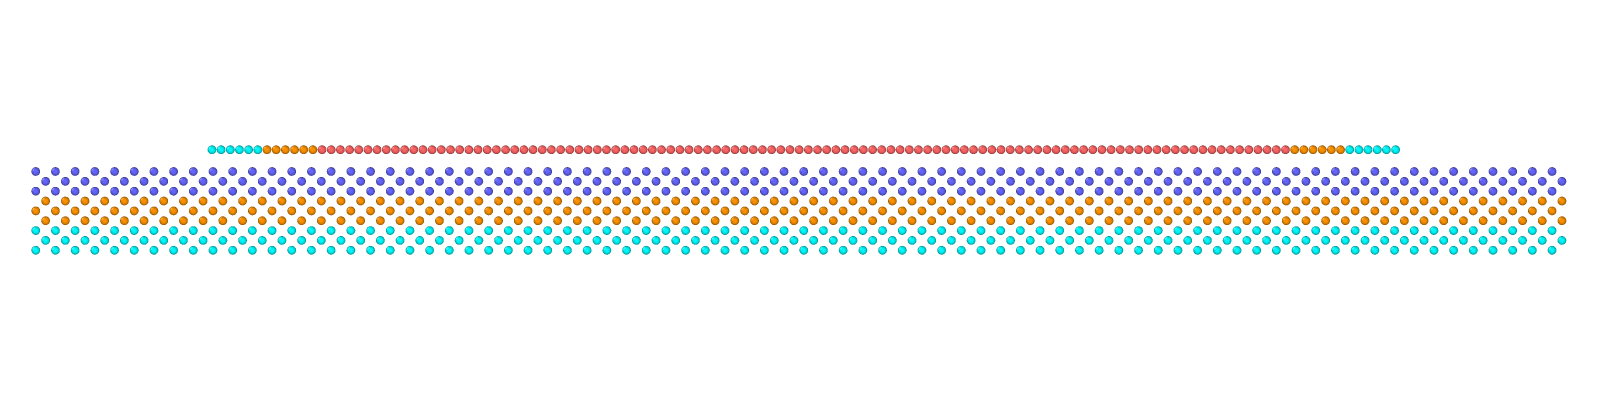
\includegraphics[width=\textwidth]{figures/system_sideview.png}
      \caption{Side view}
      \label{fig:sideview}
  \end{subfigure}
  \hfill
  \begin{subfigure}[b]{0.80\textwidth}
      \centering
      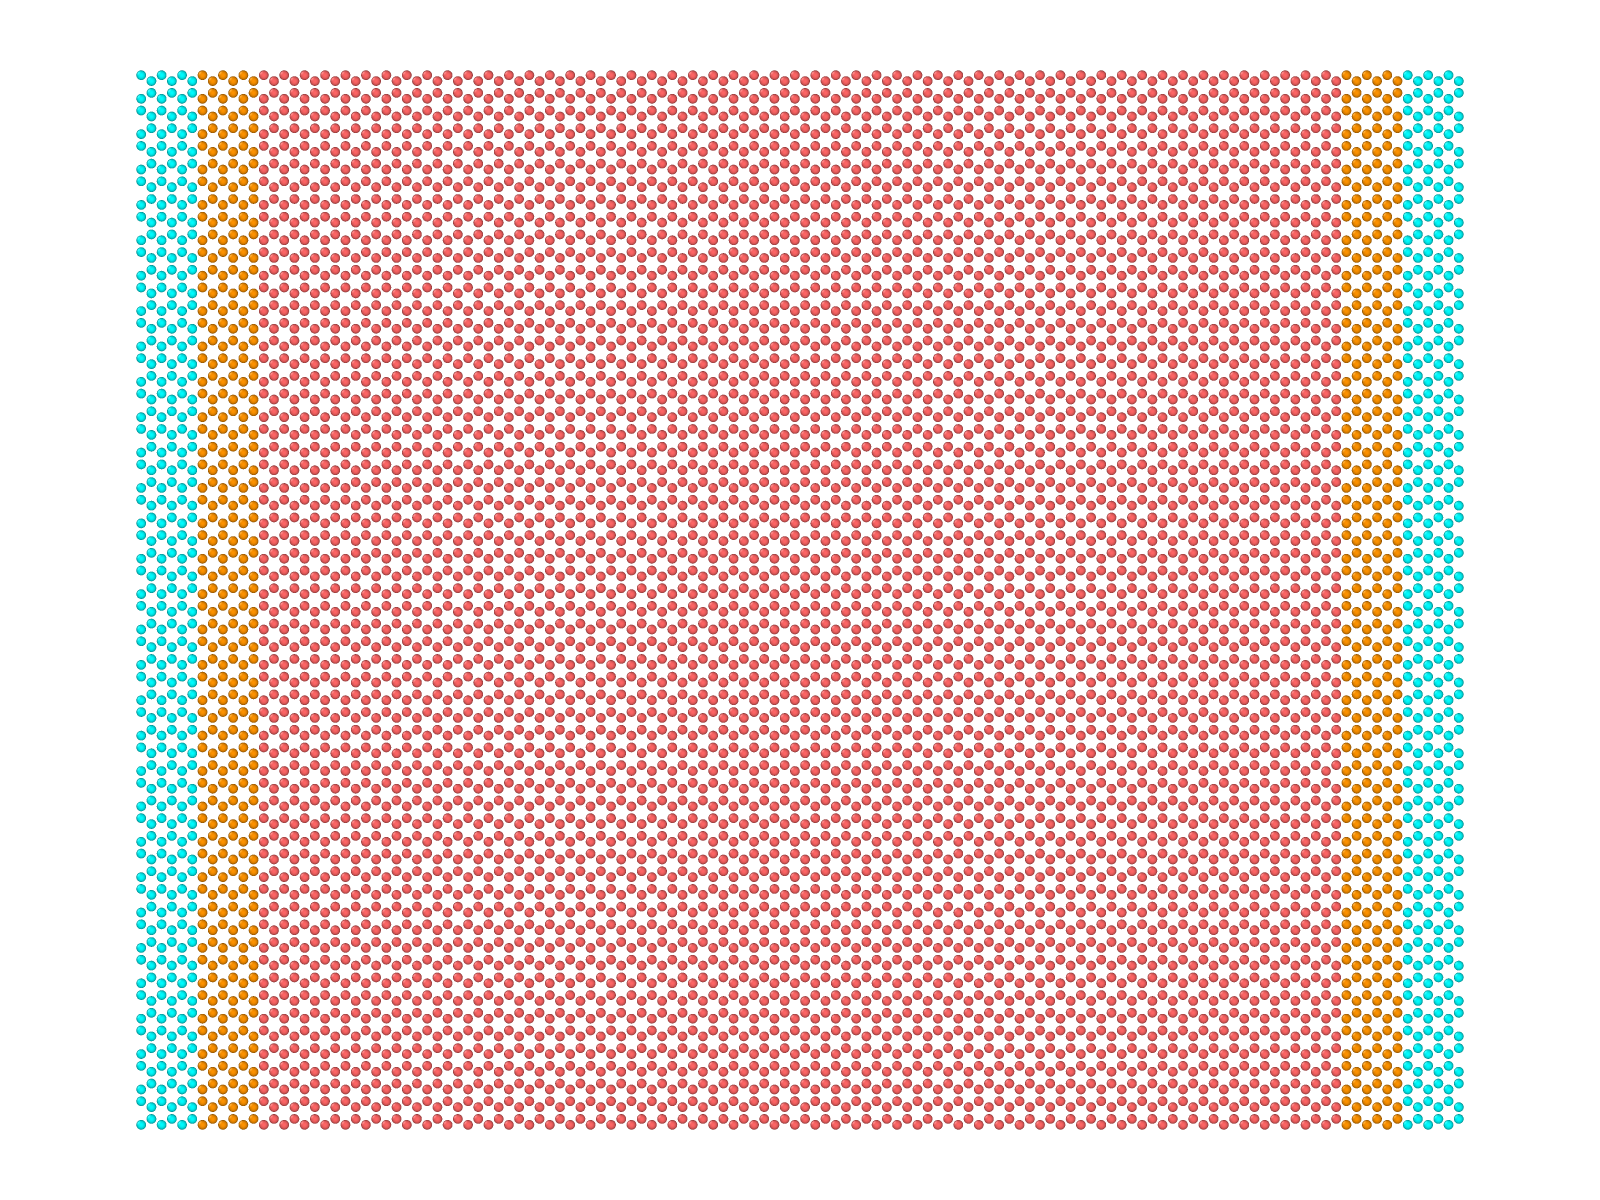
\includegraphics[width=\textwidth]{figures/system_topview.png}
      \caption{Top view}
      \label{fig:topview}
  \end{subfigure}
  \hfill
     \caption{System. 27456 atoms in total: 7272 with thermostat (orange), 7272 is locked (light blue) and the remaing 12912 just with NVE. (Get better colors)}
     \label{fig:system}
\end{figure}

% 1440 atoms in PB. 6360 atoms in inner sheet. 7800 in full sheet. 6552 in substrate freeze. 6552 atoms in group substrate_NVT. 20904 atoms in group NVE_atoms.
% 7272 atoms in group NVT_atoms. 12912 atoms in group pure_NVE.
% 7272 atoms in group locked




\begin{table}[H]
  \begin{center}
  \caption{System atom count and region division.}
  \label{tab:system_count}
  \begin{tabular}{ |c|| c | c | c | c | c | c |} \hline
    \textbf{Region} & \textbf{Total}  & Sub region & Sub total & \textbf{NVE} & \textbf{NVT} & \textbf{Locked} \\ \hline   
    \multirow{2}{*}{Sheet} & \multirow{2}{*}{7800} & Inner sheet & 6360 & 6360 & 0 & 0 \\ %\hline
    & & Pull blocks & 1440 & 0 & 720 & 720 \\ \hline   
    \multirow{2}{*}{Substrate} & \multirow{2}{*}{19656} & Upper & 6552 & 6552 & 0 & 0 \\ %\hline
    & & Middle & 6552 & 0 & 6552 & 0 \\ %\hline
    & & Bottom & 6552 & 0 & 0 & 6552 \\ \hline \hline   
    All & 27456 & \multicolumn{2}{r|}{} & 12912 & 7272 & 7272 \\ \hline 
  \end{tabular}
  \end{center}
\end{table}



% \begin{table}[ht]
%   \caption{Multi-column and multi-row table}
%   \begin{center}
%   \begin{tabular}{ccc}
%       \hline
%       \multicolumn{2}{c}{\multirow{2}{*}{Multi-col-row}}&X\\
%       \multicolumn{2}{c}{}&X\\
%       \hline
%       X&X&X\\
%       \hline
%   \end{tabular}
%   \end{center}
%   \label{tab:multicol}
%   \end{table}


% \begin{table}[H]
%   \begin{center}
%   \caption{System atom counts}
%   \label{tab:param}
%   \begin{tabular}{ | c | m{4cm}| m{4cm} | m{4cm} | m{4cm} |} \hline
%     \textbf{Region} & \textbf{Total} & \textbf{NVE} & \textbf{NVT} & \textbf{Locked} \\ \hline   
%     Full sheet (inner sheet + PB) & 
%     \begin{itemize}
%       \item[] Inner sheet: 6360
%       \item[] Pull blocks: 1440
%     \end{itemize} & 
%     \begin{itemize}
%       \item[] Inner sheet: 6360
%       \item[] Pull blocks: 1440
%     \end{itemize} & 
%     \begin{itemize}
%       \item[] Inner sheet: 0
%       \item[] Pull blocks: 720
%     \end{itemize} & 
%     \begin{itemize}
%       \item[] Inner sheet: 0
%       \item[] Pull blocks: 720
%     \end{itemize} & 
%     6360 & 720 & 720 \\ \hline   
%     Substrate & 19656 & 6552 & 6552 & 6552 \\ \hline   
%     All & 27456 & 12912 & 7272 & 7272 \\ \hline
%   \end{tabular}
%   \end{center}
% \end{table}




% m{8cm}| m{5cm}
% \begin{itemize} 
%   \item Inner sheet: 6360 
%   \item Pull blocks (PB): 1440   
% \end{itemize} 

\subsection{Creating sheets}

We are going to create a 2D sheet graphene sheet. 

\subsubsection{Graphene}
% (https://community.wvu.edu/~miholcomb/graphene.pdf) https://www.physics-in-a-nutshell.com/article/4/lattice-basis-and-crystal

Graphene is a single layer of carbon atom, graphite is the bulk, arranged in a hexagonallattice structure. We can describe the 2D crystal
structure in terms of its primitive lattice vector and a basis. That is we populate each lattice site by the given basis and translate it to
fill the whole plane by any linear combination of the lattice vectors
\begin{align*}
  \vec{T}_{mn} = m\vec{a_1} + n\vec{a_2}, \qquad m,n \in \mathbb{N}.
\end{align*}
For graphene we have the primitive lattice vectors 
\begin{align*}
  \vec{a_1} = a \left(\frac{\sqrt{3}}{2}, -\frac{1}{2}\right), \qquad \vec{a_2} = a \left(\frac{\sqrt{3}}{2}, \frac{1}{2}\right), \qquad |\vec{a_1}| = |\vec{a_2} = 2.46 \ \text{Å}.
\end{align*}
Notice that we deliberately excluded the third coordinate as we only consider a single graphene layer on not the bulk graphite consisting of
multiple layers stacked on top of each other. The basis is 
\begin{align*}
  \Big\{\Big(0,0\Big), \frac{a}{2}\Big(\frac{1}{\sqrt{3}}, 1 \Big) \Big\}
\end{align*}
It turns out that the spacing between atoms is equal for all paris with an interatomic distance 
\begin{align*}
  \left|\frac{a}{2}\Big(\frac{1}{\sqrt{3}}, 1 \Big)\right| \approx 1.42 \ \text{Å}.
\end{align*}


\begin{figure}[H]
  \centering
  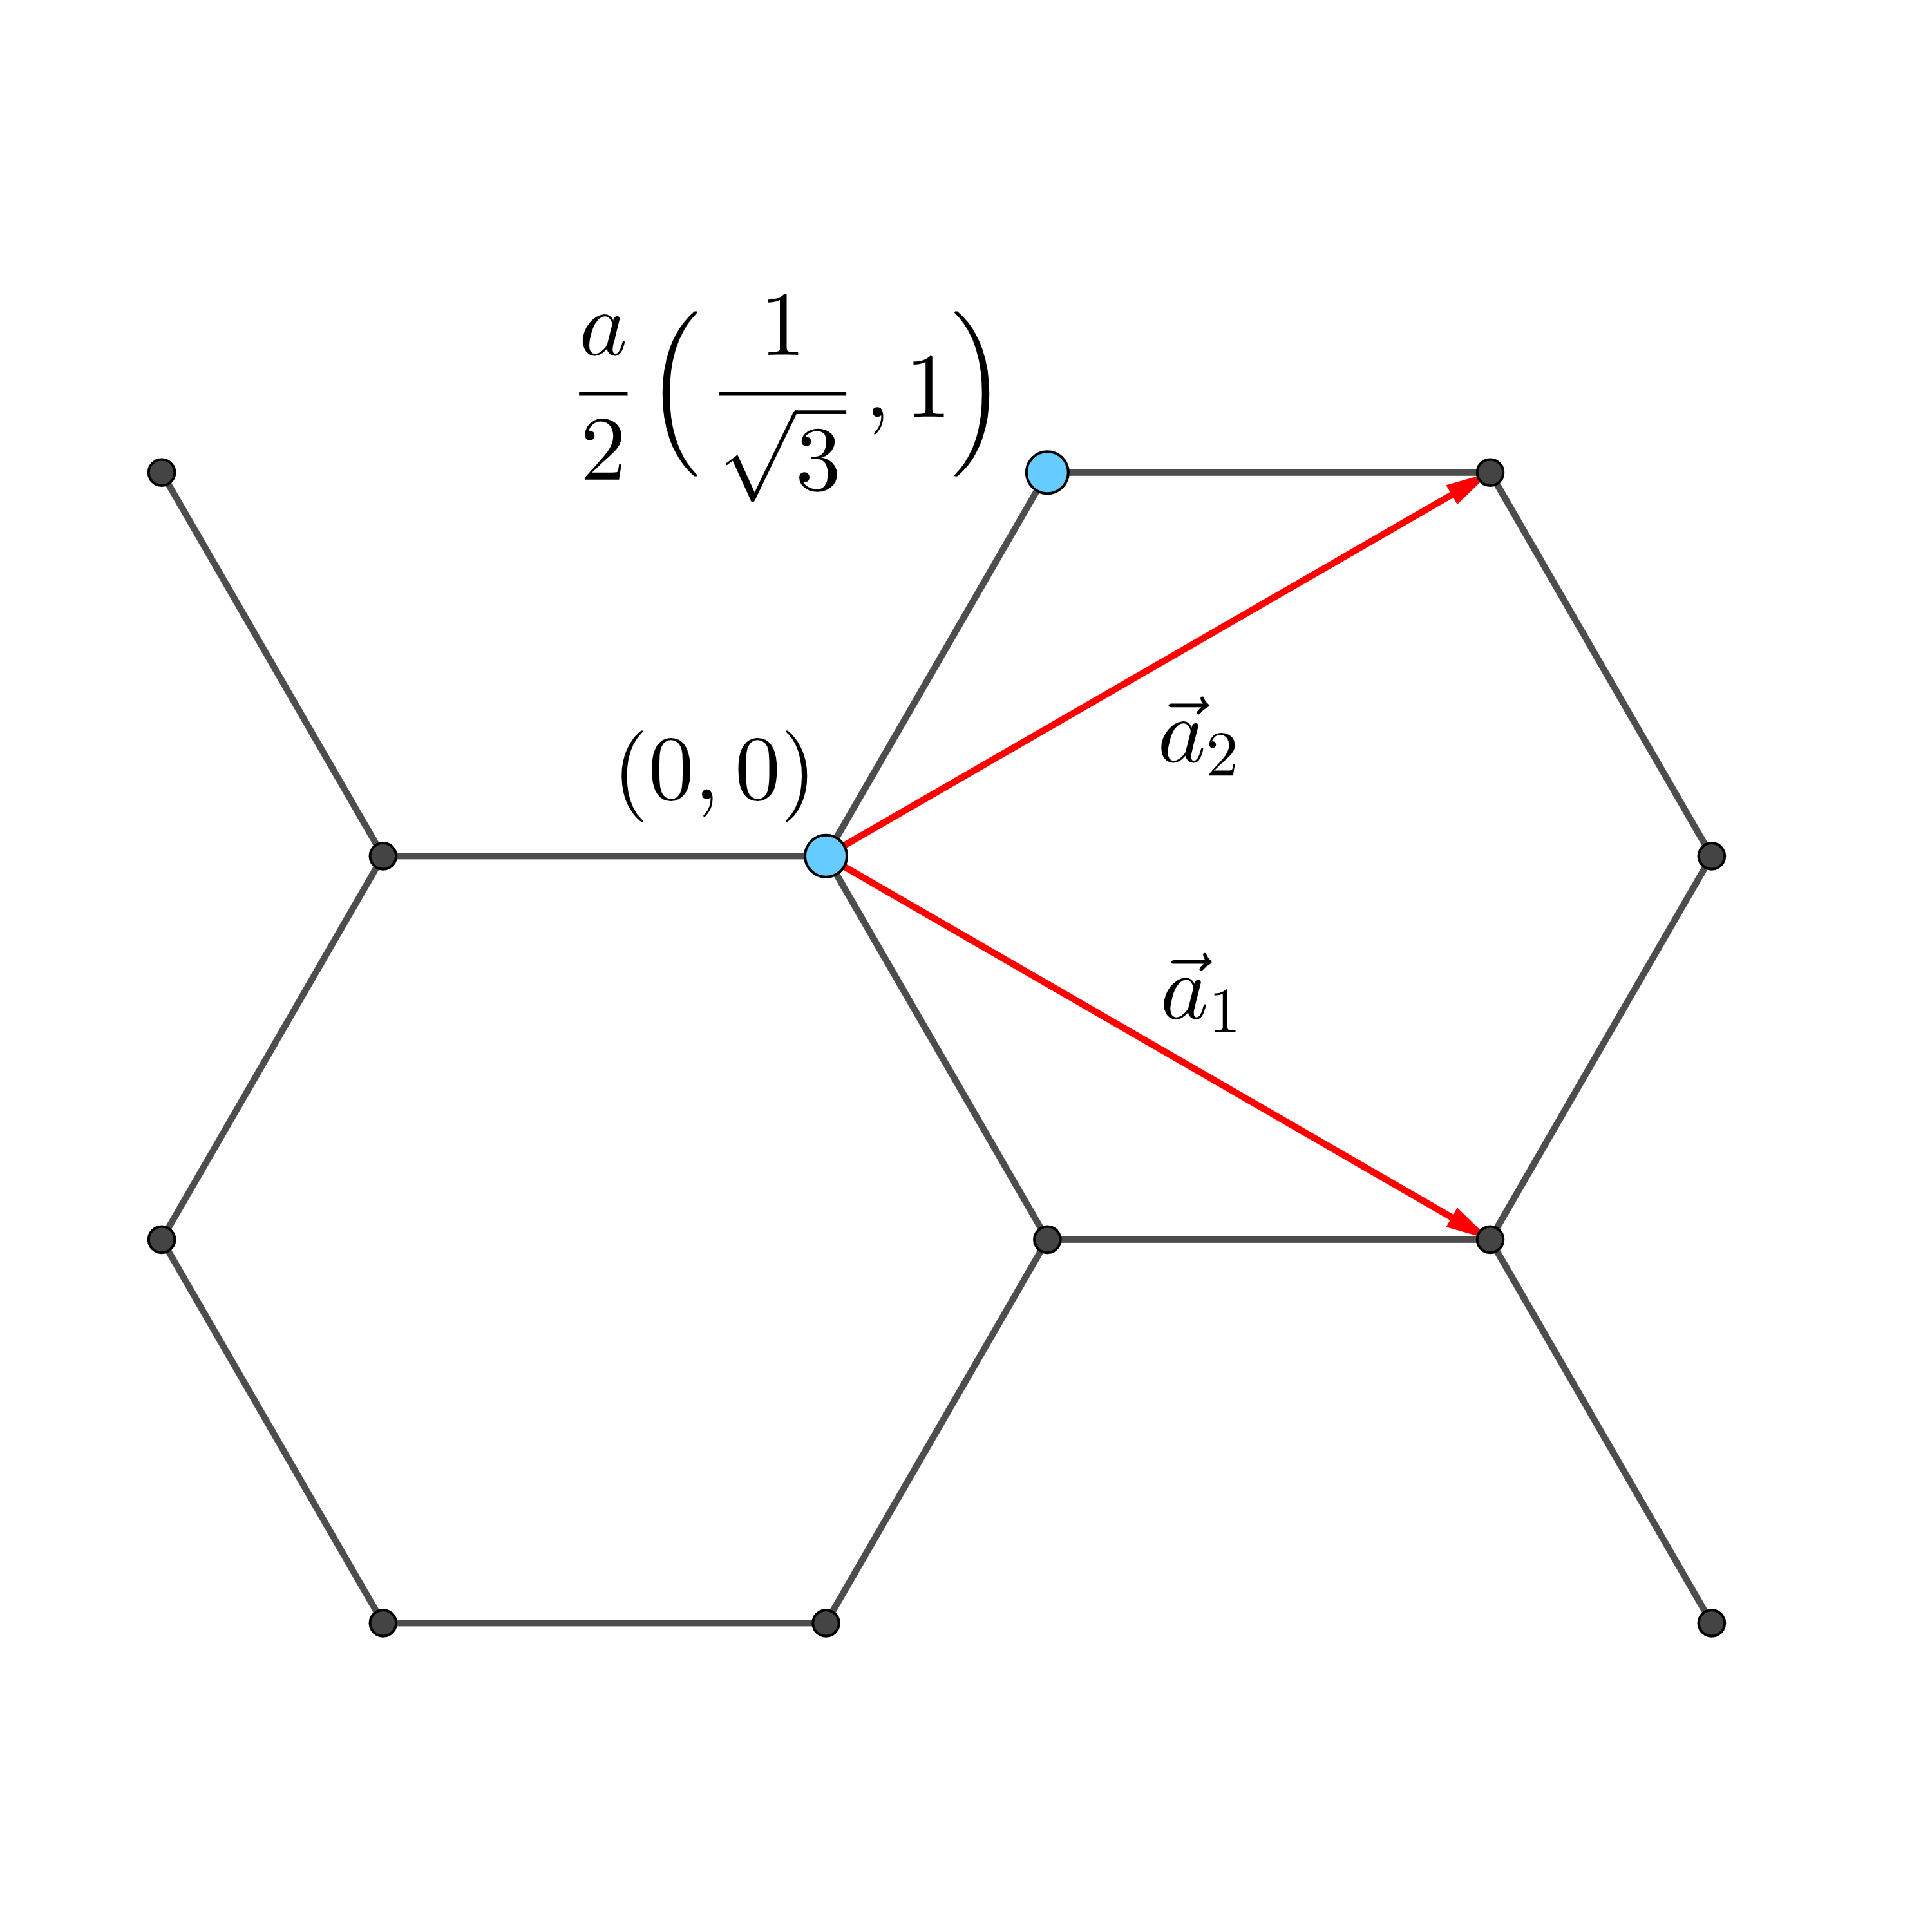
\includegraphics[width=0.3\linewidth]{figures/crystal.png}
  \caption{Graphene crystal structure with basis.}
  \label{fig:graphene_crystal}
\end{figure}



\subsubsection{Indexing}

In order to define the cut patterns applied to the graphene sheet we must define an indexing system. We must ensure that this gives an
unique description of the atoms as we eventually want to pass a binary matrix, containg 0 for removed atom and 1 for present atom, that
uniquely describes the sheet. We do this by letting the x-coordinate point to zigzag chains and the y-coordinate to the position along that
chain. This is illustrated in figure \ref{fig:atom_indexing}. Other solutions might naturally invole the lattice vectors, but as these only
can be used to translate to similar basis atoms a unfortunate duality is introduced as ones need to include the basis atom of choice into
the indexing system. With the current system we notice that locallity is somewhat preserved. That is, atom $(i, j)$ is in the proximity of
$\{(i+1, j), (i-1, j), (i, j+1), (i, j-1)\}$, but only three of them is categorized as nearest neighbours due to the hexgonal structure of
the lattice. While $(i, j\pm 1)$ is always nearest neighbours the neighbour in the x-direction flip sides with incrementing y-coordinate.
That is the nearest neighbours (NN) is decided as
\begin{align*}
  j \ \text{is even} &\rightarrow \text{NN} = \{(i+1, j), (i, j+1), (i, j-1)\}, \\
  j \ \text{is odd} &\rightarrow \text{NN} = \{(i-1, j), (i, j+1), (i, j-1)\}.
\end{align*}

\begin{figure}[H]
  \centering
  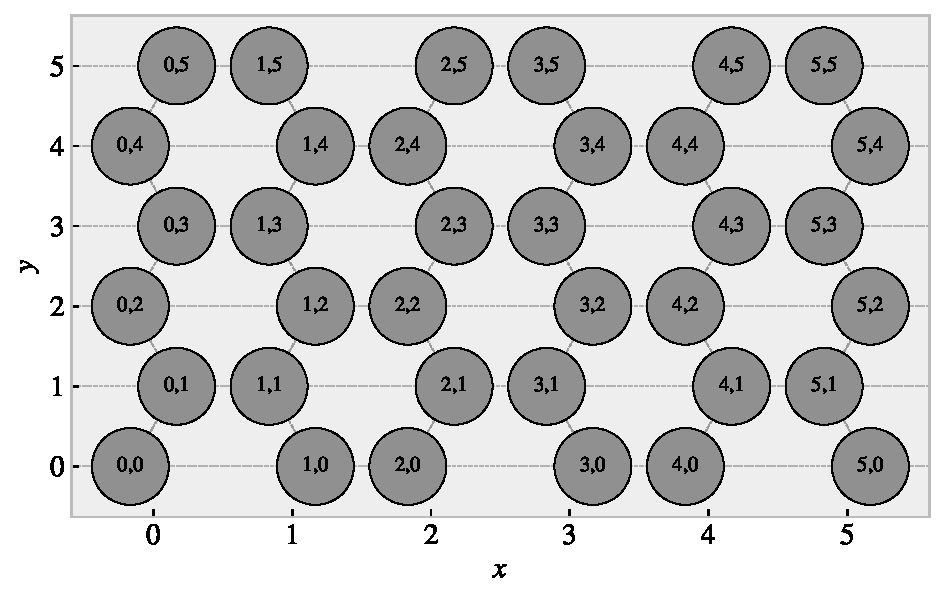
\includegraphics[width=0.7\linewidth]{figures/atom_indexing.pdf}
  \caption{Graphene atom indexing}
  \label{fig:atom_indexing}
\end{figure}

\subsubsection{Removing atoms}

As a mean to ease the formulation of cut patterns we introduce pseudo center element in each gap of the hexagonal honeycombs, see figure \ref{fig:center_indexing}. 

\begin{figure}[H]
  \centering
  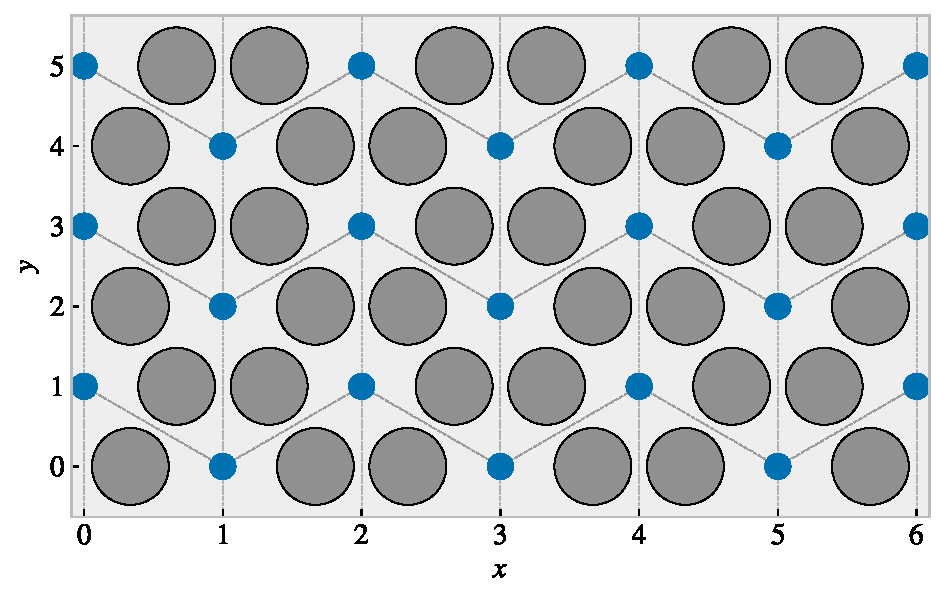
\includegraphics[width=0.7\linewidth]{figures/center_indexing.pdf}
  \caption{Graphene center indexing}
  \label{fig:center_indexing}
\end{figure}




Similar to the case of the indexing for the carbon atoms themself the nearest neighbour center elements alternate with position, this time along the x-coordinate. Each center element has six nearest neighbours, in clock wise direction we can denote them: ``up'', ``upper right'', ``lower right'', ``down'', ``lower left'', ``upper left''. The ``up'' and ``down'' is always accesed as $(i,j\pm 1)$, but for even $i$ the $(i+1,j)$ index corresponds to the ``lower right'' neighbour while for odd $i$ this corresponds to the ``upper right'' neighbour. This shifting applies for all left or right neighbours and the full neighbour list is illustrated in figure \ref{fig:center_directions}. 


\begin{figure}[H]
  \centering
  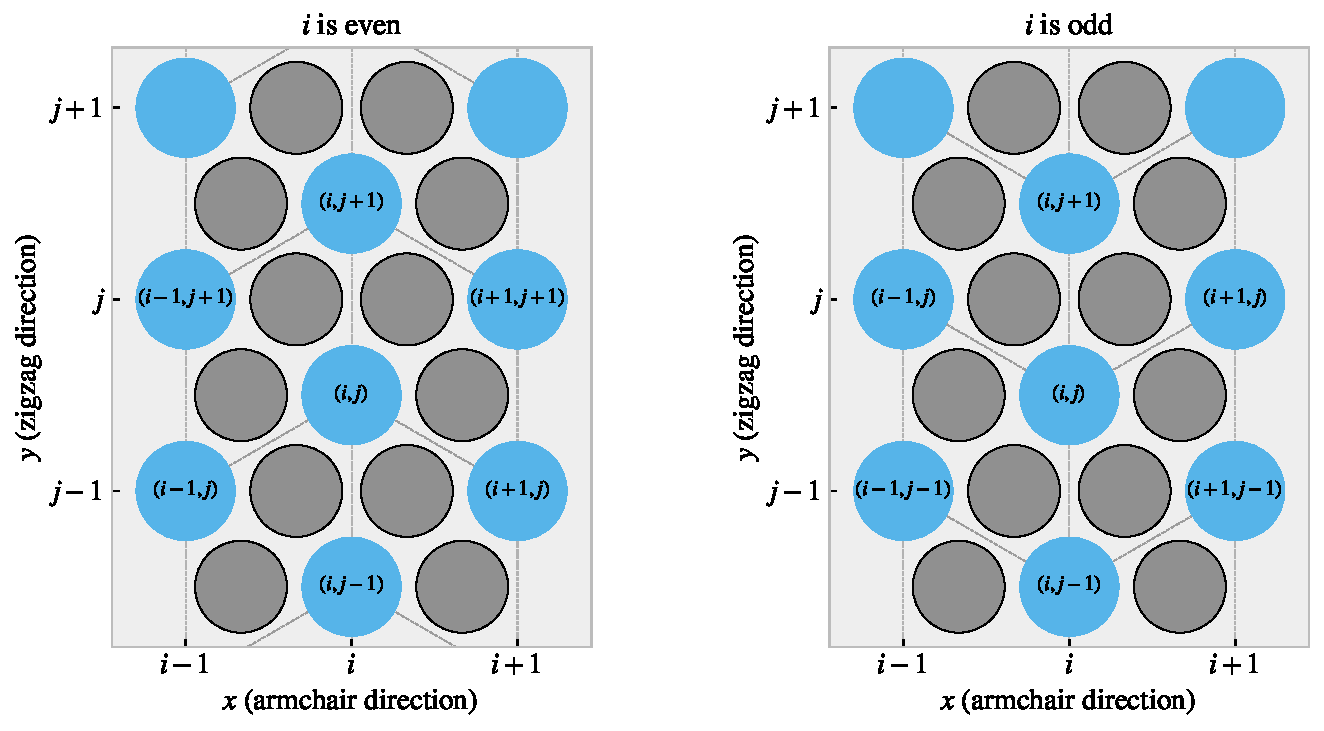
\includegraphics[width=0.7\linewidth]{figures/center_directions.pdf}
  \caption{Graphene center elements directions}
  \label{fig:center_directions}
\end{figure}


We define a cut pattern by connecting center elements into connected paths. As we walk element to element we remove atoms according to one of two rules 
\begin{enumerate}
  \item Remove intersection atoms: We remove the pair of atoms placed directly in the path we are walking. That is, when jumnping to the ``up'' center element we remove the two upper atoms located in the local hexagon of atoms. This method is sensitive to the order of the center elements in the path. 
  \item Remove all surrounding atoms: We simply remove all atoms in the local hexagon surrounding each center element. This method is indepdent of the ordering of center elements in the path.
\end{enumerate}

We notice that removing atoms using either of these rules will not garuantee an unique cut pattern. Rule 1 is the more sensitive to paths but we realize that, for an even $i$, we will remove the same five atoms following either of the following paths.
\begin{align*}
  (i, j) &\rightarrow \underbrace{(i+1,j+1)}_{\text{upper right}} \rightarrow \underbrace{(i, j+1)}_{\text{up}} \rightarrow \underbrace{(i+1, j+2)}_{\text{upperright + up}} \rightarrow \underbrace{(i+1, j+1)}_{\text{upper right}} \\
  (i, j) &\rightarrow \underbrace{(i+1,j+1)}_{\text{upper right}} \rightarrow \underbrace{(i+1, j+2)}_{\text{upperright + up}} \rightarrow \underbrace{(i, j+1)}_{\text{up}}
\end{align*}

For rule 2 it is even more abovious that different paths can result in the same atoms being removed. This is the reason that we needed to define and indexing system for the atom position itself even though that all cuts generated manually will use the center element path as reference. \\

Illustrate some delete path?




\subsubsection{Pull blocks}
\subsection{Kirigami inspired cut out patterns}
\subsubsection{Pop-up pattern}
\subsubsection{Honeycomb}
\subsubsection{Random walk}






\begin{itemize}
  \item MD simulation (classical or ab initio)
  \item Basics of classical MD simulations: Integration and stuff
  \item Ab initio simulation (quantum mechanics, solving schrödinger)
\end{itemize}
\subsection{Real life experimental procedures}
From Introduction to Tribology, Second Edition, p. 526: \par The surface force apparatus (SFA), the scanning tunneling microscopes (STM),
and atomic force and friction force microscopes (AFM and FFM) are widely used in nanotribological and nanomechanics studies.



\begin{itemize}
  \item Real life procedures to mimic in computation, for instance Atomic Force Microscoopy (AFM) for friction measurements.
  \item Available technology for test of my findings if successful (possibilities for making the nano machine) 
\end{itemize}
\subsection{Machine Learning (ML)}
\begin{itemize}
  \item Feed forward fully connected
  \item CNN
  \item GAN (encoder + decoder)
  \item Genetic algorithm
  \item Using machine learning for inverse designs partly eliminate the black box problem. When a design is produced we can test it, and if
  it works we not rely on machine learning connections to verify it's relevance. 
  \item However, using explanaitons techniques such as maybe t-SNE, Deep dream, LRP, Shapley values and linearizations, we can try to
  understand why the AI chose as it did. This can lead to an increased understanding of each design feature. Again this is not dependent on
  the complex network of the network as this can be tested and veriied independently of the network. 
\end{itemize}

\subsection{Feed forward network / Neural networks}
\subsection{CNN for image recognition}
\subsection{GAN (encoder + deoder)}
\subsection{Inverse desing using machine learning}
\subsection{Prediction explanation}
\subsubsection{Shapley}
\subsubsection{Lineariations}
\subsubsection{LRP}
\subsubsection{t-SNE}



